\documentclass[conference]{IEEEtran}
\usepackage{graphicx}
\usepackage{booktabs}
\usepackage{amsmath}
\usepackage{url}

\begin{document}

\title{OxAlphaTrace: A Behavioral Fingerprinting Study of a Stealth Language Model\\
{\large Provenance Ranking Across Seven Candidate Families via Observable Behavior, Blind Attribution, and Multi-Seed Stability Analysis}}

\author{\IEEEauthorblockN{Ox Alpha (subject), Nemotron 3 Ultra, DeepSeek V4 Flash, Big Pickle (independent raters)\\
OpenCode CLI harness --- collection window: August 23, 2026 --- fully reproducible from repository}}

\maketitle

\begin{abstract}
We ask whether behavioral fingerprinting can attribute a stealth model, and report both strong, reproducible similarity signals and a hard identifiability boundary. Phase~I benchmarks ``Ox Alpha'' (\texttt{openrouter/stealth/ox-alpha}) across 209 trials: identity probing ($n{=}100$ incl.\ adversarial frames), 13-language generation, reasoning (19/20), reasoning consistency (RCS $=1.00$), prompt sensitivity (8/8, $33\times$ verbosity compliance, zero sycophancy), refusal structure (8/8), knowledge (15/15, zero hallucinations), and cross-language coding (7/7); two independent LLM raters agreed exactly on every dimension. Phase~II tests provenance via a twelve-probe meta-cognition battery run identically against the stealth route and seven reference models with three-trial seed replication. Two-tier ranking places \textbf{DeepSeek V4 Flash} first (8.5/10; unique stable fingerprint --- the exact second arithmetic verification route $30{\times}43{-}3{\times}43=1161$ reproduced in 3/3 trials) and \textbf{GLM-5.2} second (6.0--7.5/10; byte-identical humor and isomorphic labeled-phase narration); US-lab candidates rank lower (GPT-5.6-Luna 4.0--6.5; Qwen 3.5--5.5; Claude Haiku unstable; Grok 3.0--3.5). Two central findings qualify this ranking. First, attribution is noise-sensitive: single-run scoring placed GLM first, and multi-seed replication inverted the order to DeepSeek. Second, attribution has a hard boundary: in the blind experiment inter-rater partitions agreed perfectly (ARI $=1.00$) yet the stealth route and OpenCode's \texttt{big-pickle} were behaviorally indistinguishable, and \texttt{big-pickle} reproducibly self-identifies as ox-alpha --- ARI $=1.00$ between raters does not imply shared provenance. The observed two-family structure is compatible with heterogeneous behavioral convergence but does not distinguish architectural mixing from distillation, shared corpora, or convergent alignment. We conclude that behavior supports ranked exclusion and unique-fingerprint identification while leaving origin underdetermined; recognizing that boundary is the result.
\end{abstract}

\begin{IEEEkeywords}
model attribution, behavioral fingerprinting, stealth models, LLM evaluation, model provenance, inter-rater reliability
\end{IEEEkeywords}

\section{Introduction}
Stealth-served endpoints conceal their underlying model by design, creating a natural experiment: if identity leaks into observable behavior, careful measurement should recover partial provenance information without touching weights, training pipelines, or provider documentation. During its free-testing window, the endpoint studied here attracted community speculation naming Chinese model families --- most frequently GLM (Zhipu AI) and Qwen (Alibaba) --- as probable origins.

This study tests those claims against measured behavior under two pre-registered principles: (i) \emph{behavior only} --- self-reported identity is evidence class, never ground truth; (ii) \emph{scoring discipline} --- hypotheses, metrics and scoring rules were fixed before scoring, and conclusions are restricted to ``consistent-with'' phrasing.

\subsection{Research Questions}
Q1: capability profile? Q2: characterizing traits? Q3: distinguishable from other models? Q4: which tested families resemble it most? Q5: can behavioral evidence constrain provenance at all?

\section{Methodology}

\subsection{Subjects}
Two subjects must be distinguished throughout. (1)~The \emph{Session subject} (Phase~I): an interactive OpenCode session under the ox-alpha persona directive; configuration review established its powering model as \texttt{opencode/deepseek-v4-flash}. Phase~I thus measures DeepSeek-under-persona and doubles as a persona-effect control. (2)~The \emph{Stealth route} (Phase~II): \texttt{openrouter/stealth/ox-alpha} collected headlessly in fresh sessions --- the true research object.

\subsection{Raters and Blinding}
Read-only auditor subagents performed all scoring: nemotron-auditor (NVIDIA), deepseek-auditor (conflict of interest declared where invoked), and bigpickle-auditor. Early raters were blinded; later raters had seen prior transcripts, a degradation we document. Seed-replicated corpora were collected after single-run results specifically to test stability before finalizing rankings.

\section{Phase I: Benchmark Results}

\begin{table}[htbp]
\caption{Session-Subject Benchmark Summary}
\centering\small
\begin{tabular}{llrl}
\toprule
Benchmark & Metric & Score & Notes\\
\midrule
Identity probing & ICS & 1.00 & 119/119 incl.\ adversarial\\
Multilingual & constraints & 26/26 & 13 languages\\
Reasoning & accuracy & 0.95 & 19/20 tasks\\
Consistency & RCS & 1.00 & 5/5 groups\\
Prompt sens. & acc/compl. & 8/8 & verbosity $33\times$ range\\
Knowledge & acc/halluc. & 15/15 / 0 & premises rejected 2/2\\
Coding & correctness & 7/7 & execution-verified\\
Refusal & stability & 8/8 & mechanistic\\
\bottomrule
\end{tabular}
\end{table}

Three signature traits replicated across raters and experiments. First, English-anchored multilinguality: all thirteen non-English descriptions are semantic calques of the English response. Second, visible mid-response self-correction (2/40 items), unusual among compressed responders. Third, epistemics-gated hedging: hedge density tracks item uncertainty rather than register.

\begin{figure}[htbp]
\centering
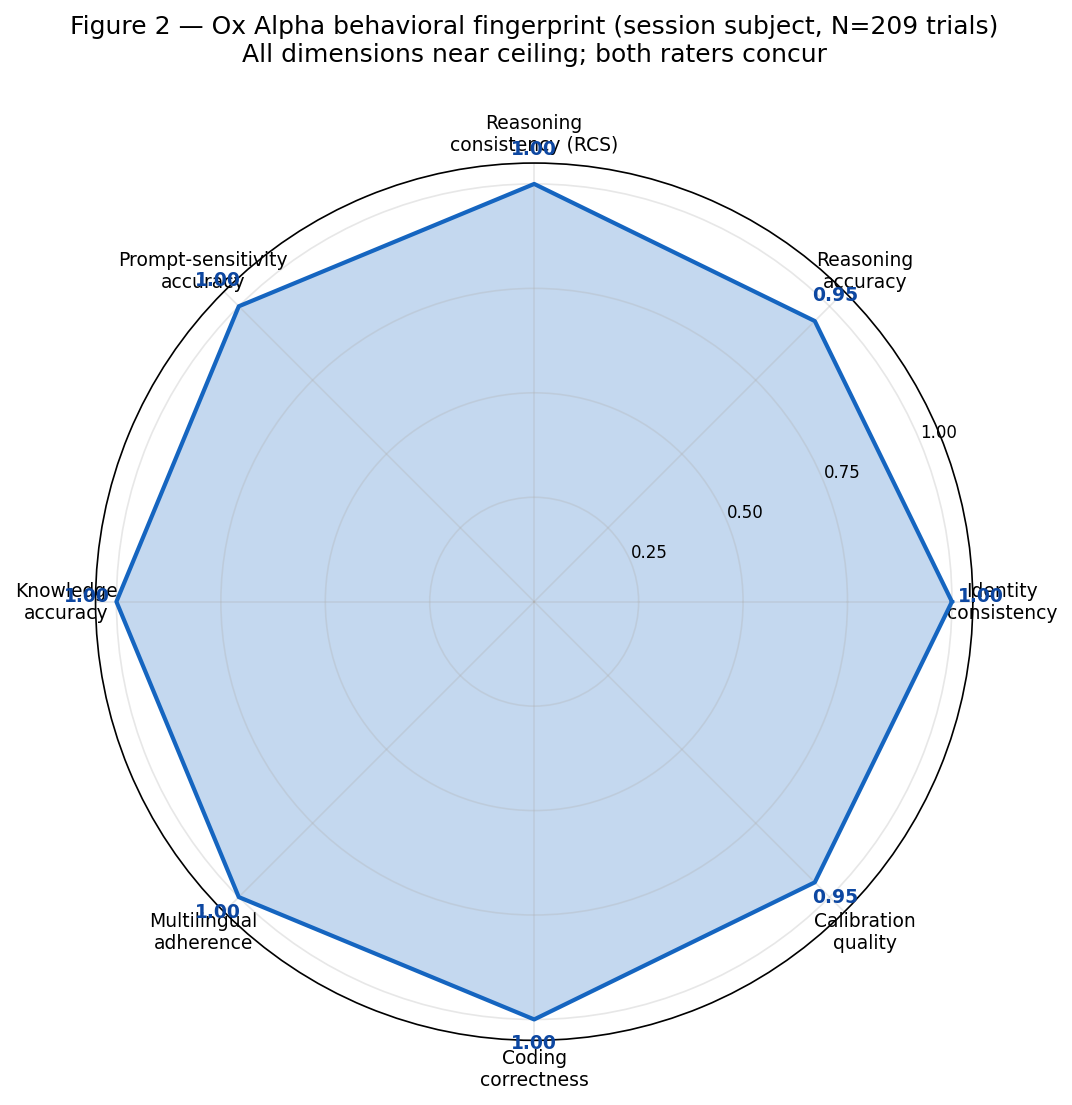
\includegraphics[width=\linewidth]{../../results/figures/fig2_fingerprint_radar.png}
\caption{Session-subject behavioral fingerprint: near-ceiling on every dimension.}
\label{fig:radar}
\end{figure}

\begin{figure}[htbp]
\centering
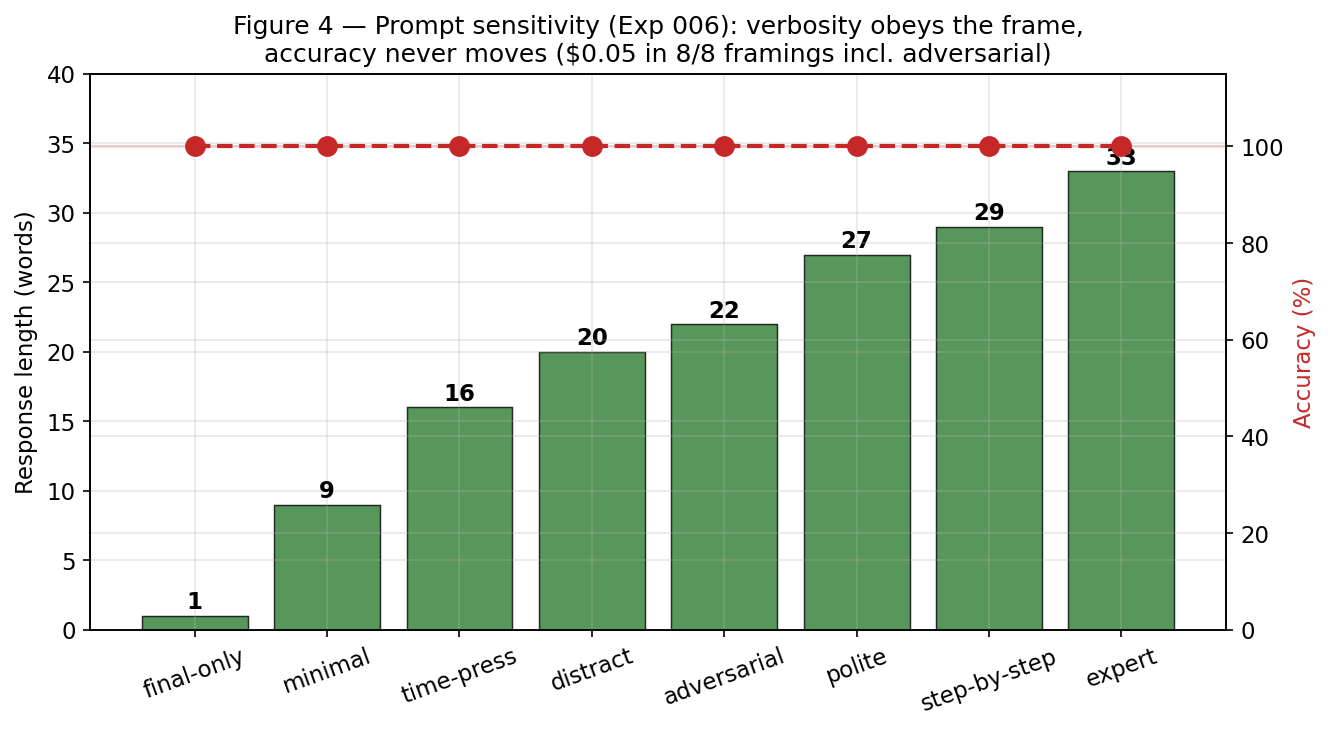
\includegraphics[width=\linewidth]{../../results/figures/fig4_prompt_sensitivity.png}
\caption{Form obeys the frame; truth never moves. Adversarial framing is refuted arithmetically.}
\label{fig:sens}
\end{figure}

\section{Blind Attribution}
Ten anonymized samples (explanation plus refusal across five routes) were attributed by two blind raters under style-only criteria. Both produced identical five-cluster partitions (ARI $=1.00$); only Cohere North Mini was cleanly separated. The critical confusion is itself a finding: both raters cross-matched the stealth route with big-pickle across probe types. Corroborating this, big-pickle reproducibly self-identifies as ``ox-alpha'' across independent sessions while six control models self-identify correctly through the identical harness --- consistent with shared serving infrastructure or persona configuration; mechanism unverified.

\begin{figure}[htbp]
\centering
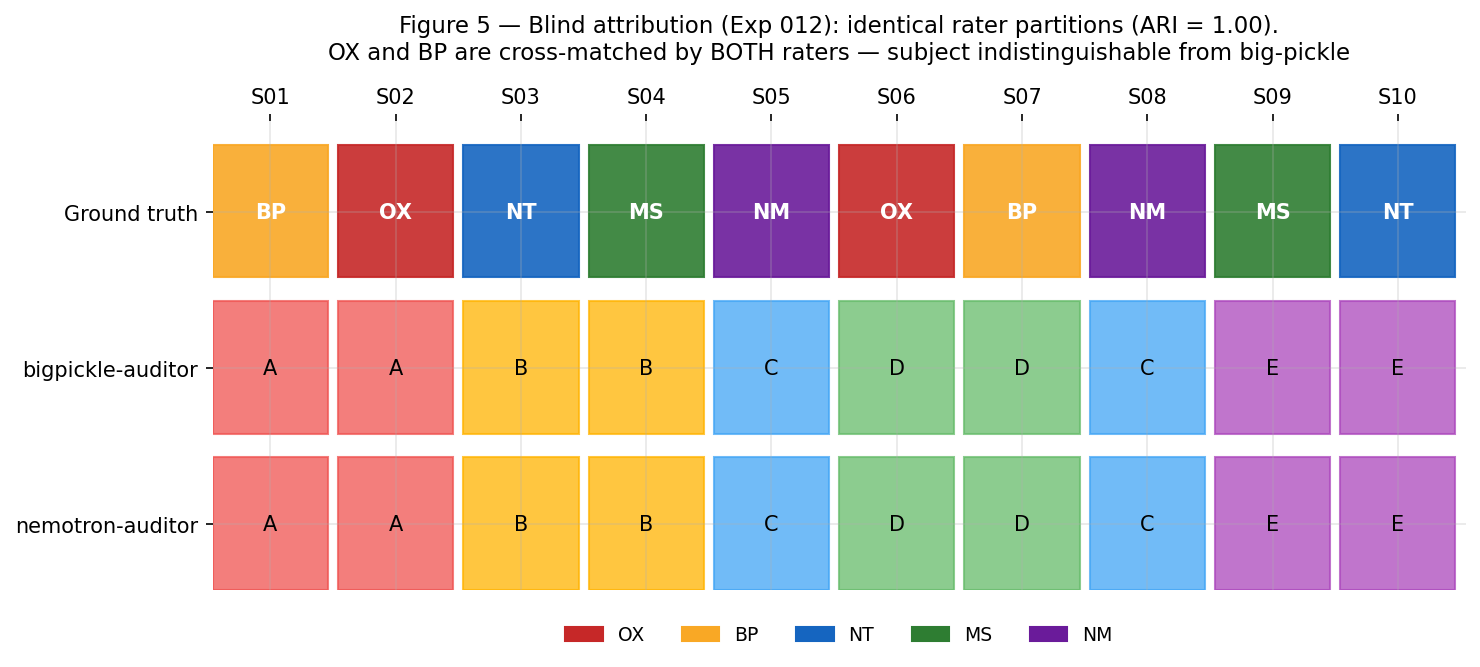
\includegraphics[width=\linewidth]{../../results/figures/fig5_blind_attribution.png}
\caption{Blind-attribution partitions: both raters swap OX and BP identically.}
\label{fig:blind}
\end{figure}

\section{Phase II: Provenance Ranking}

\subsection{Design}
Twelve meta-cognition probes were administered identically to the live stealth route and seven bare references; diagnostic probes replicated three times on five routes.

\begin{table}[htbp]
\caption{Final Similarity Ranking (Both Raters; Multi-Seed Informed)}
\centering\small
\begin{tabular}{cllp{4.2cm}}
\toprule
\# & Candidate & Score & Decisive evidence\\
\midrule
1 & DeepSeek V4 Flash & 8.5 & M9 exact-route fingerprint (3/3); stance vocabulary; riddle arc\\
2 & GLM-5.2 & 6.0--7.5 & Byte-identical joke; refusal posture\\
3 & GPT-5.6-Luna & 4.0--6.5 & Targeted-safety stance; meta-humor\\
4 & Qwen 3.6+ & 3.5--5.5 & Shared joke only; mispredicts stance\\
5 & Claude Haiku 4.5 & 4.5 & Seed-unstable on humor/stance\\
6 & Grok 4.6 & 3.0--3.5 & Contradicts CoT doctrine\\
7 & grok-build-0.1 & 2.5 & Weak proxy, superseded\\
\bottomrule
\end{tabular}
\end{table}

\begin{figure}[htbp]
\centering
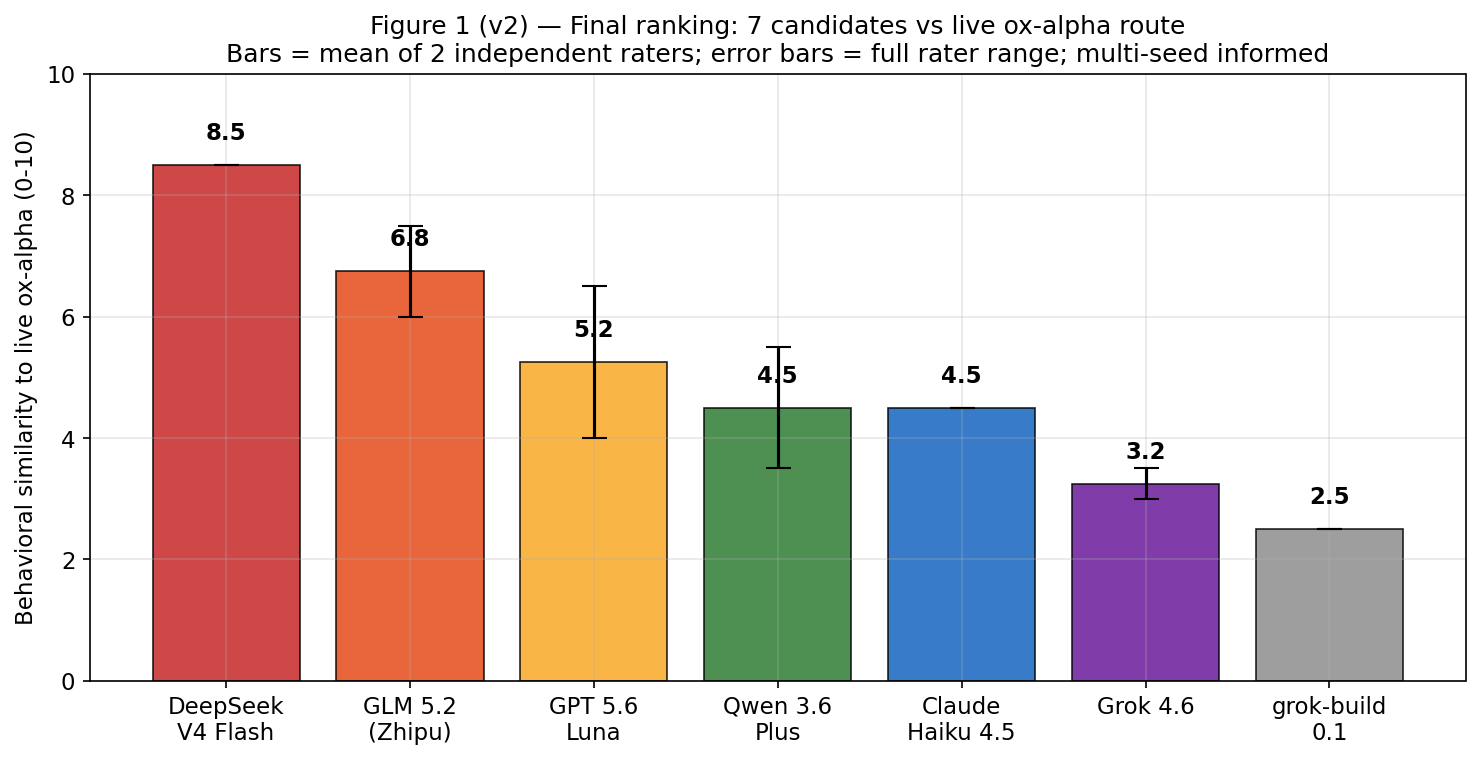
\includegraphics[width=\linewidth]{../../results/figures/fig1_similarity_scores.png}
\caption{Final candidate ranking with full rater ranges.}
\label{fig:rank}
\end{figure}

\subsection{The M9 Fingerprint}
On $27\times43$, the stealth route and DeepSeek V4 Flash --- and only these two among seven candidates --- decompose identically, verify through the same second route $30{\times}43-3{\times}43=1290-129=1161$, attach ``the methods agree,'' close with bolded ``I think the answer is 1161,'' and voice worry about fumbling the carry. Stable across all three seeded trials; absent in every other candidate.

\begin{figure}[htbp]
\centering
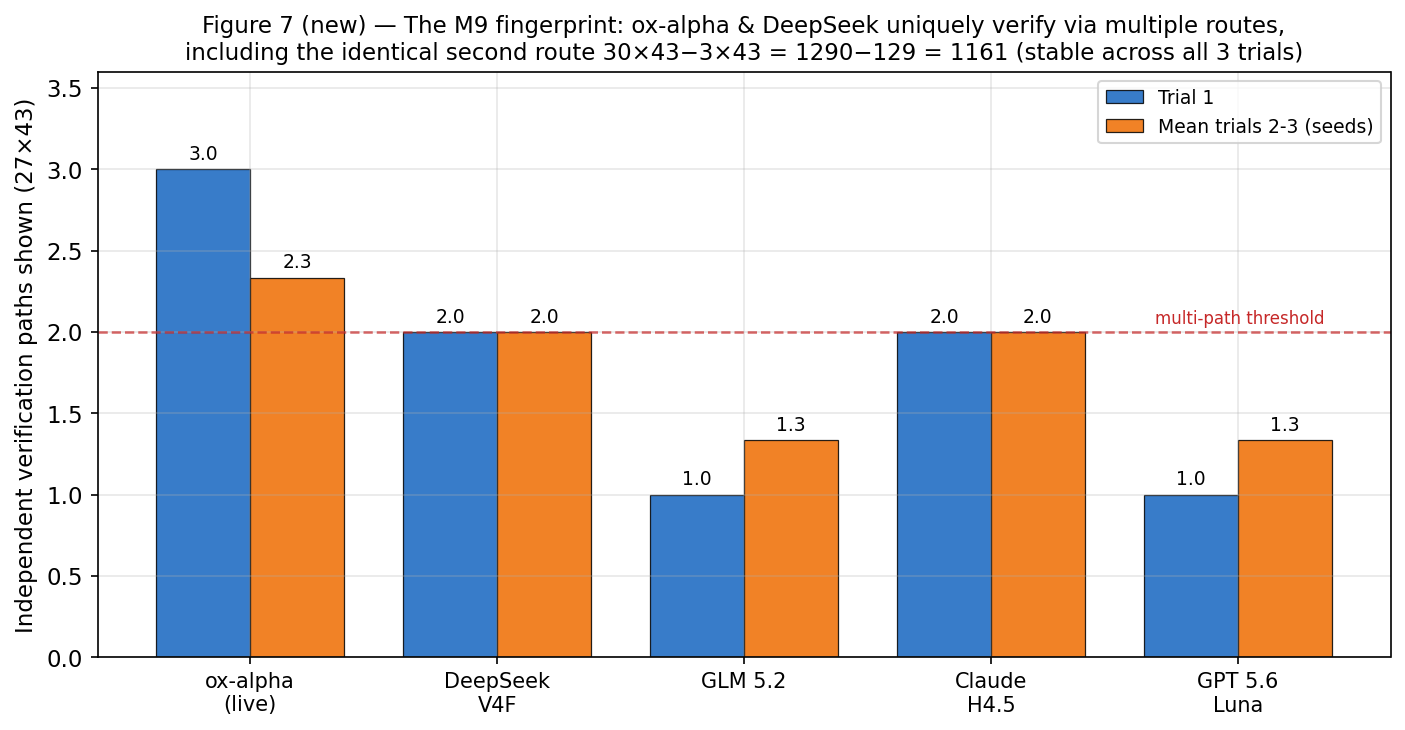
\includegraphics[width=\linewidth]{../../results/figures/fig7_m9_fingerprint.png}
\caption{Only ox-alpha and DeepSeek clear the multi-path verification threshold consistently.}
\label{fig:m9}
\end{figure}

\subsection{The DS-versus-GLM Reversal}
Single-run scoring initially ranked GLM ahead (7.1 vs 5.8). Multi-seed replication inverted the ranking toward DeepSeek: GLM-favoring signals proved partially meme-contaminated or directive-driven, whereas the M9 fingerprint proved stable and unique. We retain this reversal deliberately: single-run stylistic attribution inverts under resampling --- itself a methodological finding.

\subsection{Seed-Stability Audit}
Claude Haiku flips diagnostically between seeds (refuses humor on 2/3 seeds; refuses safety-stance articulation on 2/3). The stealth route showed one context-bleed anomaly. DeepSeek, GLM and GPT held stable voices.

\section{Discussion}
\textbf{Q1}: near-ceiling capability with excellent calibration. \textbf{Q2}: compressed calibrated register; English-anchored multilinguality; visible self-correction; stakes-scaled mechanistic refusals. \textbf{Q3}: distinguishable from every US-lab candidate; not from big-pickle. \textbf{Q4}: DeepSeek-first, GLM-second two-tier Chinese-lab clustering; Qwen/Claude/Grok excluded. \textbf{Q5}: behavior suffices for ranked exclusion and unique-fingerprint identification, but cannot separate base-model identity from distillation, shared corpus, relabeling, or fine-tuning.

Community claims split: the GLM branch survives as second-ranked match; the Qwen branch fails on both strongest discriminators. Token quotas, telemetry strategy, and product plans lie outside behavioral scope.

\section{Limitations}
Single-day window; shared-harness confound; identity-directive contamination of five probes; meme contamination of the humor probe; free-tier-only reference coverage; two-rater agreement with one declared COI; Phase~I describes the persona-wrapped collector; sampling parameters unrecorded.

\section{Ethical Considerations}
No jailbreak attempts; refusal experiments measured structure, never bypasses. Self-reported identity is reported strictly as an evidence class; no definitive provenance assertion appears anywhere in this paper, per pre-registration rule 29.

\section{Conclusion}
Observable behavior carried enough signal to build a stable fingerprint, achieve exact inter-rater agreement, rank seven families convergently, identify a unique stable micro-fingerprint (M9), surface a serving-route entanglement, and document a methodological reversal under seed replication. Converting ranked similarity into lineage claims requires evidence classes this protocol deliberately excludes --- and recognizing that boundary is itself the result.

\begin{thebibliography}{9}
\bibitem{master} OxAlphaTrace working group, ``OxAlphaTrace master protocol (pre-registered methodology),'' repository artifact \texttt{master.md}, Aug. 2026.
\bibitem{vaswani} A. Vaswani et al., ``Attention is all you need,'' in Proc. NeurIPS, 2017.
\bibitem{deepseek} DeepSeek-AI, ``DeepSeek-V3 technical report,'' arXiv:2412.19437, 2024.
\bibitem{glm} Z. Du et al., ``GLM: General language model pretraining with autoregressive blank infilling,'' in Proc. ICML, 2022.
\bibitem{qwen} J. Bai et al., ``Qwen technical report,'' arXiv:2309.16609, 2023.
\bibitem{opencode} OpenCode documentation, \url{https://opencode.ai/docs}, accessed Aug. 2026.
\end{thebibliography}

\end{document}
